% Options for packages loaded elsewhere
\PassOptionsToPackage{unicode}{hyperref}
\PassOptionsToPackage{hyphens}{url}
\PassOptionsToPackage{dvipsnames,svgnames,x11names}{xcolor}
\documentclass[
  11pt,
]{article}
\usepackage{xcolor}
\usepackage[margin=2.5cm]{geometry}
\usepackage{amsmath,amssymb}
\setcounter{secnumdepth}{-\maxdimen} % remove section numbering
\usepackage{iftex}
\ifPDFTeX
  \usepackage[T1]{fontenc}
  \usepackage[utf8]{inputenc}
  \usepackage{textcomp} % provide euro and other symbols
\else % if luatex or xetex
  \usepackage{unicode-math} % this also loads fontspec
  \defaultfontfeatures{Scale=MatchLowercase}
  \defaultfontfeatures[\rmfamily]{Ligatures=TeX,Scale=1}
\fi
\usepackage[]{charter}
\ifPDFTeX\else
  % xetex/luatex font selection
\fi
% Use upquote if available, for straight quotes in verbatim environments
\IfFileExists{upquote.sty}{\usepackage{upquote}}{}
\IfFileExists{microtype.sty}{% use microtype if available
  \usepackage[]{microtype}
  \UseMicrotypeSet[protrusion]{basicmath} % disable protrusion for tt fonts
}{}
\makeatletter
\@ifundefined{KOMAClassName}{% if non-KOMA class
  \IfFileExists{parskip.sty}{%
    \usepackage{parskip}
  }{% else
    \setlength{\parindent}{0pt}
    \setlength{\parskip}{6pt plus 2pt minus 1pt}}
}{% if KOMA class
  \KOMAoptions{parskip=half}}
\makeatother
\usepackage{graphicx}
\makeatletter
\newsavebox\pandoc@box
\newcommand*\pandocbounded[1]{% scales image to fit in text height/width
  \sbox\pandoc@box{#1}%
  \Gscale@div\@tempa{\textheight}{\dimexpr\ht\pandoc@box+\dp\pandoc@box\relax}%
  \Gscale@div\@tempb{\linewidth}{\wd\pandoc@box}%
  \ifdim\@tempb\p@<\@tempa\p@\let\@tempa\@tempb\fi% select the smaller of both
  \ifdim\@tempa\p@<\p@\scalebox{\@tempa}{\usebox\pandoc@box}%
  \else\usebox{\pandoc@box}%
  \fi%
}
% Set default figure placement to htbp
\def\fps@figure{htbp}
\makeatother
\setlength{\emergencystretch}{3em} % prevent overfull lines
\providecommand{\tightlist}{%
  \setlength{\itemsep}{0pt}\setlength{\parskip}{0pt}}
% ==========================================================================
%  IA na Sociedade — cabeçalho LaTeX (pdflatex)
%  Programa CiberExt 26-29 · FEELT38103
%  Adaptado de "AI in Society" (Universidade de Helsinque / Una Europa)
%  Licença: CC BY-NC-SA 4.0
% --------------------------------------------------------------------------
%  Espelha a identidade do ia-style.css: papel quente, tinta ardósia e a
%  faixa tricolor dos três eixos do curso (conceitos / aplicações / riscos).
% ==========================================================================

% ---------- Fontes ----------
% A serifada vem do build.sh, que passa  -V fontfamily=charter  ao pandoc.
% Aqui só acrescentamos a sem-serifa; ambas com fallback, porque nem toda
% instalação de LaTeX traz os mesmos pacotes.
\IfFileExists{helvet.sty}{\usepackage[scaled=0.90]{helvet}}{}
\usepackage{textcomp}
\IfFileExists{microtype.sty}{\usepackage{microtype}}{}

% ---------- Pacotes de layout ----------
\usepackage{xcolor}
\usepackage{tcolorbox}
\tcbuselibrary{skins,breakable}
\usepackage{titlesec}
\usepackage{fancyhdr}
\usepackage{enumitem}
\usepackage{amssymb}
\usepackage{booktabs}
\usepackage{array}
\usepackage{colortbl}
\usepackage{ragged2e}
\usepackage{fvextra}
\usepackage{newunicodechar}

% ---------- Caracteres Unicode que o pdflatex não conhece ----------
\newunicodechar{✓}{{\color{iaAplic}\checkmark}}
\newunicodechar{✅}{{\color{iaAplic}\checkmark}}
\newunicodechar{→}{\ensuremath{\rightarrow}}
\newunicodechar{←}{\ensuremath{\leftarrow}}
\newunicodechar{↔}{\ensuremath{\leftrightarrow}}
\newunicodechar{–}{--}
\newunicodechar{—}{---}
\newunicodechar{€}{\texteuro}
\newunicodechar{£}{\textsterling}
\newunicodechar{×}{\ensuremath{\times}}
\newunicodechar{≈}{\ensuremath{\approx}}
\newunicodechar{≥}{\ensuremath{\geq}}
\newunicodechar{≤}{\ensuremath{\leq}}
\newunicodechar{•}{\textbullet}
\newunicodechar{″}{''}
\newunicodechar{′}{'}

% ==========================================================================
%  PALETA — os mesmos valores do ia-style.css
% ==========================================================================
\definecolor{iaConceitos}{HTML}{24505C}   % petróleo — títulos, eixo 1
\definecolor{iaAplic}{HTML}{16746C}       % verdete  — subtítulos, eixo 2
\definecolor{iaRiscos}{HTML}{B45F14}      % açafrão  — destaques, eixo 3
\definecolor{iaAmeixa}{HTML}{77345F}      % links internos, termos técnicos
\definecolor{iaTinta}{HTML}{1F2933}       % corpo do texto
\definecolor{iaTintaFraca}{HTML}{5C6670}
\definecolor{iaRegra}{HTML}{E4DBCD}
\definecolor{iaBloco}{HTML}{F3EEE4}
\definecolor{iaNota}{HTML}{EAF1F0}
\definecolor{iaCaso}{HTML}{FCF3E6}
\definecolor{iaFilos}{HTML}{F7EFF4}

\color{iaTinta}

% ==========================================================================
%  ASSINATURA — faixa tricolor dos três eixos
% ==========================================================================
\newcommand{\faixaEixos}[1][\linewidth]{%
  \noindent
  \textcolor{iaConceitos}{\rule{0.3333#1}{4pt}}%
  \textcolor{iaAplic}{\rule{0.3333#1}{4pt}}%
  \textcolor{iaRiscos}{\rule{0.3333#1}{4pt}}%
  \par}

% ---------- Página de título ----------
\makeatletter
\newcommand{\subtitle}[1]{\gdef\@subtitle{#1}}
\providecommand{\@subtitle}{}
\def\@maketitle{%
  \newpage\null\vskip 1.5em%
  \faixaEixos
  \vskip 2.2em
  {\raggedright
    {\sffamily\bfseries\huge\color{iaConceitos}\@title\par}%
    \vskip 0.7em%
    {\sffamily\large\color{iaTintaFraca}\@subtitle\par}%
    \vskip 2em%
    {\color{iaRegra}\rule{\linewidth}{1pt}}%
    \vskip 1em%
    {\sffamily\small\color{iaTinta}\@author\par}%
    \vskip 0.5em%
    {\sffamily\footnotesize\color{iaTintaFraca}\@date\par}%
  }\par\vskip 2.5em}
\makeatother

% ==========================================================================
%  TÍTULOS DE SEÇÃO
% ==========================================================================
\titleformat{\section}[block]
  {\sffamily\Large\bfseries\color{iaConceitos}}
  {\thesection}{0.7em}{}
  [{\vspace{2pt}\color{iaRegra}\titlerule[1.2pt]}]
\titleformat{\subsection}
  {\sffamily\large\bfseries\color{iaAplic}}
  {\thesubsection}{0.6em}{}
\titleformat{\subsubsection}
  {\sffamily\normalsize\bfseries\color{iaRiscos}}
  {\thesubsubsection}{0.5em}{}
\titleformat{\paragraph}[runin]
  {\sffamily\small\bfseries\color{iaRiscos}}
  {}{0em}{}

\titlespacing*{\section}{0pt}{2.6ex plus 1ex minus .2ex}{1.3ex plus .2ex}
\titlespacing*{\subsection}{0pt}{2.2ex plus 1ex minus .2ex}{1ex plus .2ex}

% ==========================================================================
%  CABEÇALHO E RODAPÉ
% ==========================================================================
\setlength{\headheight}{24pt}
\renewcommand{\sectionmark}[1]{\markboth{#1}{}}
\pagestyle{fancy}
\fancyhf{}
\renewcommand{\headrulewidth}{0.6pt}
\renewcommand{\footrulewidth}{0pt}
\fancyhead[L]{\sffamily\footnotesize\color{iaAplic}Ética da IA}
\fancyhead[R]{\sffamily\footnotesize\color{iaAplic}\nouppercase{\leftmark}}
\fancyfoot[C]{\sffamily\footnotesize\color{iaConceitos}\thepage}
\renewcommand{\headrule}{%
  \hbox to\headwidth{\color{iaRegra}\leaders\hrule height \headrulewidth\hfill}}

% ==========================================================================
%  TEXTO CORRIDO
% ==========================================================================
\linespread{1.08}
\setlength{\parskip}{0.55em}
\setlength{\parindent}{0pt}
\emergencystretch=3em
\hbadness=10000

% ---------- Termos técnicos / código inline ----------
\let\oldtexttt\texttt
\renewcommand{\texttt}[1]{{\color{iaAmeixa}\small\ttfamily #1}}

% ---------- Blocos verbatim ----------
\fvset{breaklines=true,breakanywhere=true,fontsize=\small}

% ---------- Blocos de código (ambiente Shaded do pandoc) ----------
% O pandoc só pré-define o ambiente Shaded quando o markdown tem bloco de
% código; nos capítulos sem código ele não existe, e \renewenvironment
% incondicional falharia com "Environment Shaded undefined". \@ifundefined
% escolhe \newenvironment ou \renewenvironment conforme o caso.
\makeatletter
\@ifundefined{Shaded}{\newenvironment{Shaded}}{\renewenvironment{Shaded}}
  {\begin{tcolorbox}[
      breakable, enhanced jigsaw, rounded corners,
      arc=3pt, boxrule=0pt, frame hidden,
      colback=iaBloco,
      borderline west={3pt}{0pt}{iaAmeixa},
      left=10pt, right=8pt, top=6pt, bottom=6pt,
      before skip=9pt, after skip=9pt]}
  {\end{tcolorbox}}
\makeatother

% ---------- Citações: caixa de caso ----------
\renewenvironment{quote}
  {\begin{tcolorbox}[
      breakable, enhanced jigsaw, rounded corners,
      arc=3pt, boxrule=0pt, frame hidden,
      colback=iaCaso,
      borderline west={3pt}{0pt}{iaRiscos},
      left=12pt, right=10pt, top=9pt, bottom=9pt,
      before skip=9pt, after skip=9pt]}
  {\end{tcolorbox}}

% ==========================================================================
%  BLOCOS DE APOIO
%  No markdown, escreva:   ::: nota   ...texto...   :::
%  O pandoc converte fenced_divs para os ambientes abaixo.
% ==========================================================================
\newtcolorbox{iabox}[3]{
  breakable, enhanced jigsaw, rounded corners,
  arc=3pt, boxrule=0pt, frame hidden,
  colback=#2,
  borderline west={3pt}{0pt}{#1},
  left=12pt, right=10pt, top=9pt, bottom=9pt,
  before skip=11pt, after skip=11pt,
  before upper={\setlength{\parskip}{0.5em}\setlength{\parindent}{0pt}},
  title={\sffamily\bfseries\footnotesize\textcolor{#1}{\MakeUppercase{#3}}},
  attach title to upper={\par\vspace{5pt}},
  fonttitle=\normalfont}

% Cada ambiente aceita um titulo opcional entre colchetes, vindo do
% atributo data-titulo do markdown:   \begin{filosofia}[Titulo] ... \end{filosofia}
% Os quatro primeiros espelham os icones do material original.
\newenvironment{filosofia}[1][Conceito filosofico]{\begin{iabox}{iaAmeixa}{iaFilos}{#1}}{\end{iabox}}
\newenvironment{tecnica}[1][Nota tecnica]{\begin{iabox}{iaConceitos}{iaNota}{#1}}{\end{iabox}}
\newenvironment{contexto}[1][Contexto]{\begin{iabox}{iaAplic}{iaBloco}{#1}}{\end{iabox}}
\newenvironment{definicao}[1][Definicao]{\begin{iabox}{iaRiscos}{iaCaso}{#1}}{\end{iabox}}

\newenvironment{nota}[1][Nota]{\begin{iabox}{iaConceitos}{iaNota}{#1}}{\end{iabox}}
\newenvironment{caso}[1][Caso]{\begin{iabox}{iaRiscos}{iaCaso}{#1}}{\end{iabox}}
\newenvironment{reflexao}[1][Para pensar]{\begin{iabox}{iaAplic}{iaBloco}{#1}}{\end{iabox}}
\newenvironment{licenca}
  {\par\vspace{2em}\faixaEixos\par\vspace{0.8em}
   \begingroup\sffamily\scriptsize\color{iaTintaFraca}}
  {\endgroup\par}

% ==========================================================================
%  LISTAS
% ==========================================================================
\setlist[itemize]{leftmargin=1.4em, itemsep=2pt, topsep=4pt, parsep=0pt}
\setlist[enumerate]{leftmargin=1.7em, itemsep=2pt, topsep=4pt, parsep=0pt}
\renewcommand{\labelitemi}{\textcolor{iaRiscos}{\textbullet}}
\renewcommand{\labelitemii}{\textcolor{iaAplic}{--}}

% ==========================================================================
%  TABELAS
% ==========================================================================
\renewcommand{\arraystretch}{1.3}
\arrayrulecolor{iaRegra}

% ==========================================================================
%  RÓTULOS EM PORTUGUÊS
%  Definidos aqui (e não via -V na linha de comando) porque acentos passados
%  como argumento dependem do locale do terminal e podem se corromper.
% ==========================================================================
\renewcommand{\contentsname}{Sumário}
\renewcommand{\refname}{Referências}
\renewcommand{\figurename}{Figura}
\renewcommand{\tablename}{Tabela}
\usepackage{bookmark}
\IfFileExists{xurl.sty}{\usepackage{xurl}}{} % add URL line breaks if available
\urlstyle{same}
% fallback for those not using the hyperref driver hyperxmp:
\makeatletter
\@ifundefined{xmpquote}{\newcommand{\xmpquote}[1]{#1}}{}
\makeatother
\hypersetup{
  pdftitle={Ética da Inteligência Artificial},
  colorlinks=true,
  linkcolor={iaAmeixa},
  filecolor={Maroon},
  citecolor={Blue},
  urlcolor={iaRiscos},
  pdfcreator={LaTeX via pandoc}}

\title{Ética da Inteligência Artificial}
\usepackage{etoolbox}
\makeatletter
\providecommand{\subtitle}[1]{% add subtitle to \maketitle
  \apptocmd{\@title}{\par {\large #1 \par}}{}{}
}
\makeatother
\subtitle{Capítulo 2: Não-maleficência --- o que devemos fazer?}
\author{Tradução e adaptação para o português: José Lucas Lira Bizil,
Fernando Mazzeto Lisboa Lima e Matheus da Silva Fernandes\\
Programa CiberExt 26-29 · FEELT38103 · Universidade Federal de
Uberlândia\\
Original: \emph{Ethics of AI}, Universidade de Helsinque}
\date{2026}

\begin{document}
\maketitle

{
\hypersetup{linkcolor=iaConceitos}
\setcounter{tocdepth}{3}
\tableofcontents
}
\section{Capítulo 2: Não-maleficência --- o que devemos
fazer?}\label{capuxedtulo-2-nuxe3o-maleficuxeancia-o-que-devemos-fazer}

\begin{nota}[Sobre este capítulo]

\textbf{Eixo:} Conceitos e Riscos

O que significa ``fazer o bem'' e ``não causar dano'' quando falamos de
IA? Este capítulo apresenta o utilitarismo --- uma das respostas
filosóficas clássicas para a pergunta sobre o bem comum --- e também
seus limites.

\end{nota}

\subsection{I. O que devemos fazer?}\label{i.-o-que-devemos-fazer}

\subsubsection{O princípio da
beneficência}\label{o-princuxedpio-da-beneficuxeancia}

\begin{quote}
\emph{``A IA inevitavelmente se enreda nas dimensões éticas e políticas
das vocações e práticas em que está inserida. A ética da IA é, na
prática, um microcosmo dos desafios políticos e éticos enfrentados pela
sociedade.''}

Brent Mittelstadt
\end{quote}

O princípio da \textbf{beneficência} diz ``faça o bem'', enquanto o
princípio da \textbf{não-maleficência} afirma ``não cause dano''. Embora
esses dois princípios possam parecer semelhantes, representam princípios
distintos. A beneficência incentiva a criação de uma IA benéfica (``a IA
deve ser desenvolvida para o bem comum e o benefício da humanidade''),
ao passo que a não-maleficência diz respeito às consequências negativas
e aos riscos da IA.

De modo geral, a ética da IA tem se ocupado principalmente do princípio
da não-maleficência. A discussão concentrou-se sobretudo em como
desenvolvedores, fabricantes, autoridades e outras partes interessadas
devem minimizar os riscos éticos --- discriminação, proteção da
privacidade, danos físicos e sociais --- que podem surgir de aplicações
de IA. Com frequência, essas discussões são formuladas em termos de uso
indevido intencional, invasão maliciosa, medidas técnicas ou estratégias
de gestão de risco.

\begin{filosofia}[O solucionismo tecnológico]

Críticos afirmam que a ênfase na não-maleficência transforma a ética
numa questão de encontrar soluções técnicas para problemas técnicos. Os
problemas morais passam a ser vistos como coisas que podem ser
resolvidas por ``consertos'' técnicos, ou apenas por um bom projeto.
Esquece-se o contexto ético e social mais amplo em que os sistemas
técnicos estão inseridos. Muitas questões importantes que orientam o
controle, a governança e as dimensões sociais da IA são ignoradas.

O pesquisador de tecnologia Evgeny Morozov chama isso de ``solucionismo
tecnológico'' (\emph{tech solutionism}) --- a convicção de que problemas
causados pela tecnologia sempre podem ser resolvidos com mais
tecnologia.

\end{filosofia}

Como resultado, problemas éticos profundos e difíceis são simplificados
demais e ficam sem resposta. Uma dessas questões é o problema do ``bem
comum''. O que exatamente isso significa? Neste capítulo, examinaremos
uma resposta filosófica clássica.

\subsection{II. O bem comum --- calculando
consequências}\label{ii.-o-bem-comum-calculando-consequuxeancias}

\begin{figure}
\centering
\pandocbounded{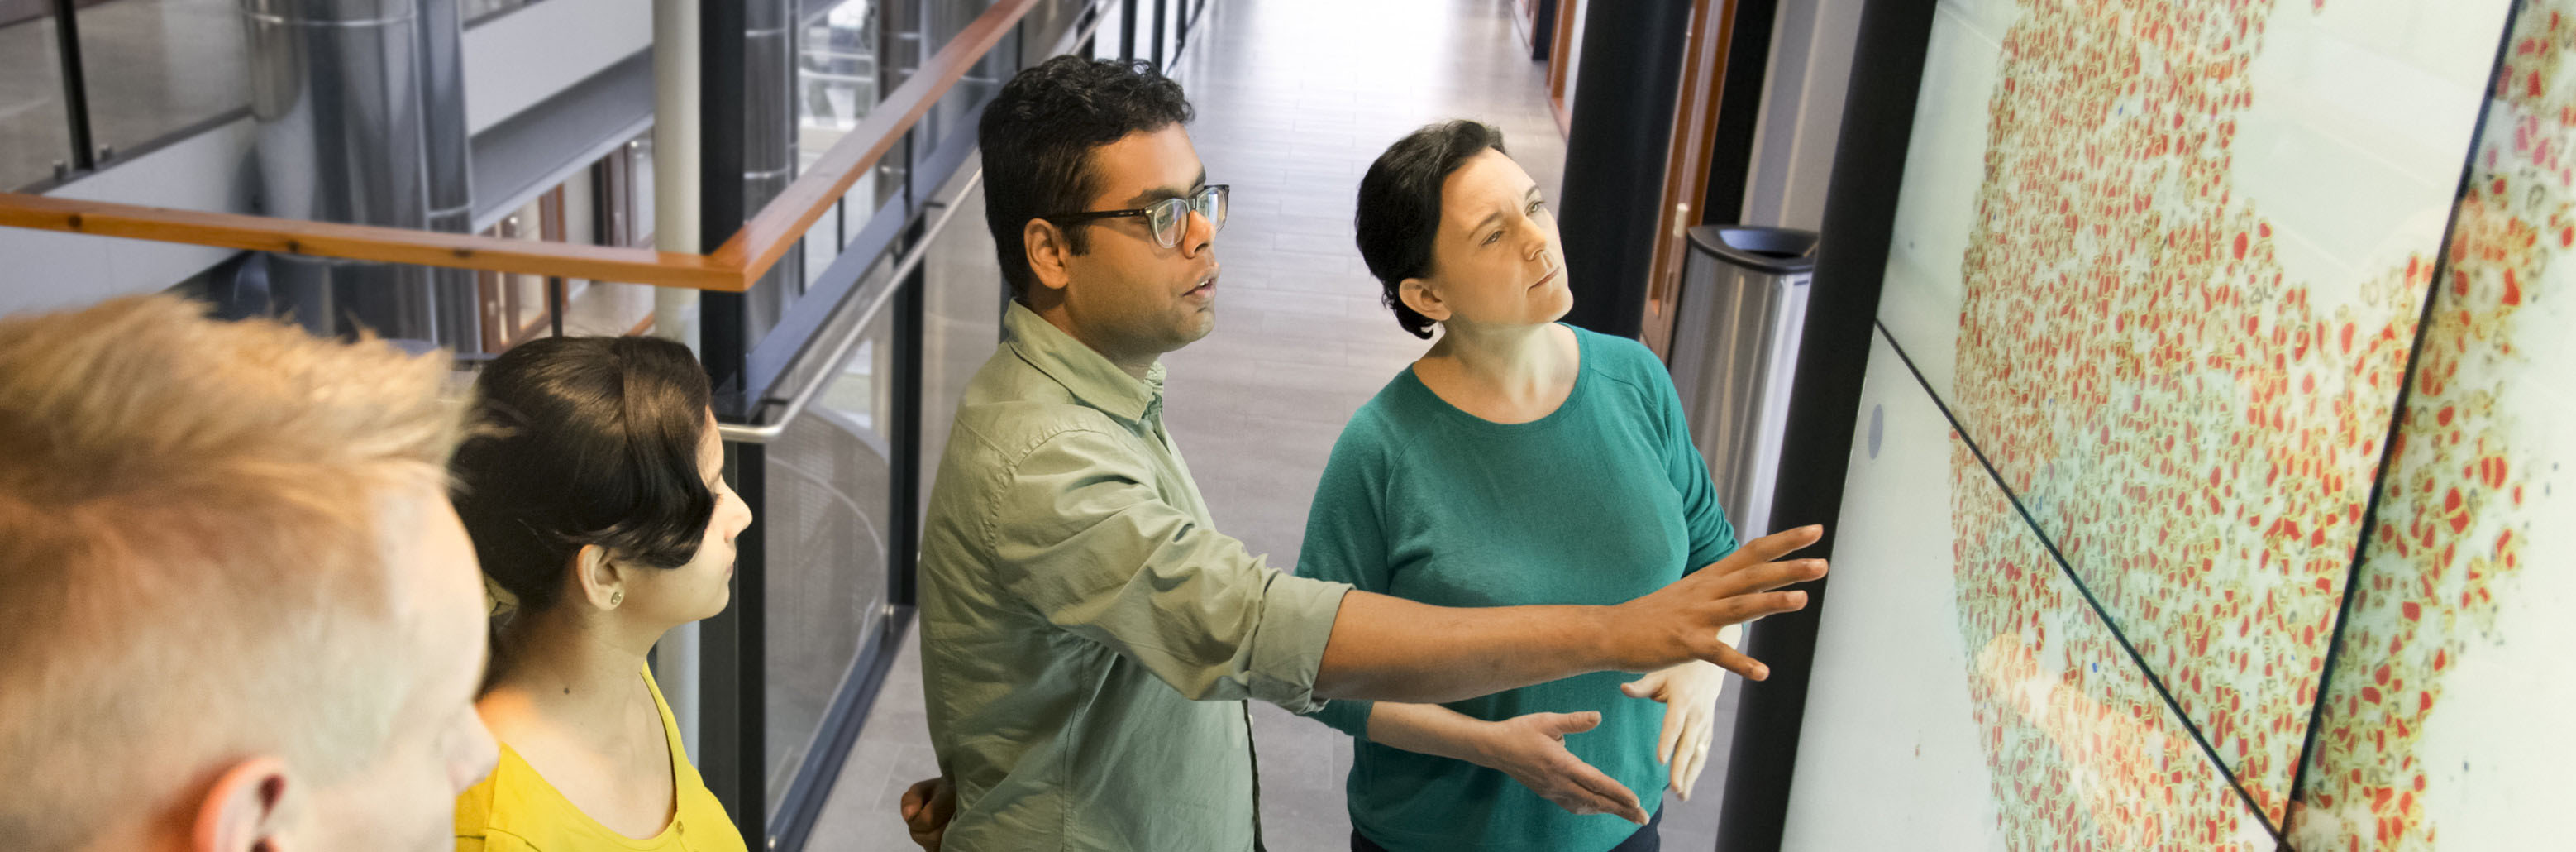
\includegraphics[keepaspectratio,alt={Ilustração}]{img/stk_keksi_hki_biomedicum_0129_cropped.jpg}}
\caption{Ilustração}
\end{figure}

\emph{Ilustração. © Keksi Agency via Cidade de Helsinque / Comunicação}

Suponha que você seja o diretor digital (\emph{Chief Digital Officer})
da cidade de Helsinque. Pedem que você avalie se a organização de saúde
da cidade deveria migrar de uma saúde ``reativa'' para uma saúde
``preventiva''. Você lê um relatório. Ele fala de sistemas de
aprendizado de máquina (\emph{machine learning}) novos e sofisticados
que ajudariam as autoridades de saúde a prever os possíveis riscos de
saúde dos cidadãos.

Esses métodos produzem previsões combinando e analisando diversas fontes
de dados médicos e de sistemas de saúde. Analisando um grande número de
critérios, indivíduos de alto risco poderiam ser identificados e
priorizados. Essas pessoas poderiam ser convidadas proativamente a uma
consulta médica para receber o tratamento adequado.

\textbf{Os benefícios}

O relatório menciona muitas vantagens. Por exemplo, a prevenção de
doenças tem grande potencial de melhorar a saúde e a qualidade de vida
dos cidadãos. Além disso, permitiria melhor estimativa de impacto e
melhor planejamento dos serviços básicos de saúde. A saúde preventiva
também tem potencial de reduzir significativamente os custos sociais e
de saúde. Essas economias, enfatiza o relatório, poderiam ser usadas
para o bem comum.

\textbf{Os problemas potenciais}

O relatório, porém, também traz algumas preocupações. Por exemplo, os
sistemas levantam uma série de questões jurídicas e éticas relativas à
privacidade, à segurança e ao uso dos dados. O relatório pergunta, por
exemplo: onde fica a fronteira entre prevenção aceitável e intrusão
inaceitável? A cidade tem direito de usar dados médicos privados e
sensíveis para identificar pacientes de alto risco? Como deve ser dado o
consentimento, e o que acontecerá com as pessoas que não o derem? E
quanto às pessoas que não dão consentimento porque não são capazes de
fazê-lo?

O relatório levanta ainda a questão fundamental do papel da cidade: se a
cidade tem informação sobre um risco potencial de saúde e não age sobre
esses dados, a cidade é culpada de negligência? Os cidadãos são tratados
igualmente nos mundos físico e digital? Se uma pessoa desmaia na vida
real, chamamos uma ambulância sem ter permissão explícita para isso. No
mundo digital, preocupações com privacidade podem nos impedir de
contatar os cidadãos.

O que você acha do exemplo acima? Como diretor digital, você promoveria
o uso de métodos preventivos? Se sua resposta for algo como ``sim, a
cidade deveria buscar uma forma ética e juridicamente aceitável de usar
esses métodos --- há tantas vantagens em comparação com os possíveis
riscos'', você provavelmente estava usando uma forma de raciocínio moral
chamada ``utilitarismo''.

\begin{definicao}[Utilitarismo]

\textbf{Utilitarismo} é uma família de teorias éticas. Ela concebe
``benefícios'' como ações que maximizam o bem-estar de todos os
indivíduos afetados. O utilitarismo é uma versão do consequencialismo,
que afirma que as consequências de qualquer ação são os únicos padrões
do certo e do errado.

\end{definicao}

Segundo os utilitaristas, as ações moralmente corretas são aquelas que
produzem o maior saldo de benefícios sobre danos para todos os afetados.
Diferentemente de outras formas mais individualistas de
consequencialismo (como o egoísmo) ou de consequencialismos com pesos
desiguais (como o prioritarismo), o utilitarismo considera igualmente os
interesses de todos os seres humanos. Contudo, os utilitaristas divergem
em muitas questões específicas, como saber se as ações devem ser
escolhidas com base em seus resultados prováveis (utilitarismo de ato)
ou se os agentes devem se conformar a regras que maximizem a utilidade
(utilitarismo de regra). Há também divergência sobre se deve ser
maximizada a utilidade total (utilitarismo total), a média (utilitarismo
médio) ou a mínima.

Para os utilitaristas, a utilidade --- ou benefício --- é definida em
termos de bem-estar ou felicidade. Por exemplo, Jeremy Bentham, o pai do
utilitarismo, caracterizou a utilidade como ``aquela propriedade
{[}\ldots{]} que tende a produzir benefício, vantagem, prazer, bem ou
felicidade {[}\ldots{]} ou a impedir que ocorram dano, dor, mal ou
infelicidade à parte cujo interesse está sendo considerado.''

O utilitarismo oferece um método relativamente simples para decidir se
uma ação é moralmente correta ou não. Para descobrir o que devemos
fazer, seguimos estes passos:

\begin{itemize}
\tightlist
\item
  primeiro, identificamos as várias ações que poderíamos realizar;
\item
  segundo, estimamos os benefícios e os danos que resultariam de cada
  ação;
\item
  terceiro, escolhemos a ação que oferece os maiores benefícios depois
  de considerados os custos.
\end{itemize}

\begin{figure}
\centering
\pandocbounded{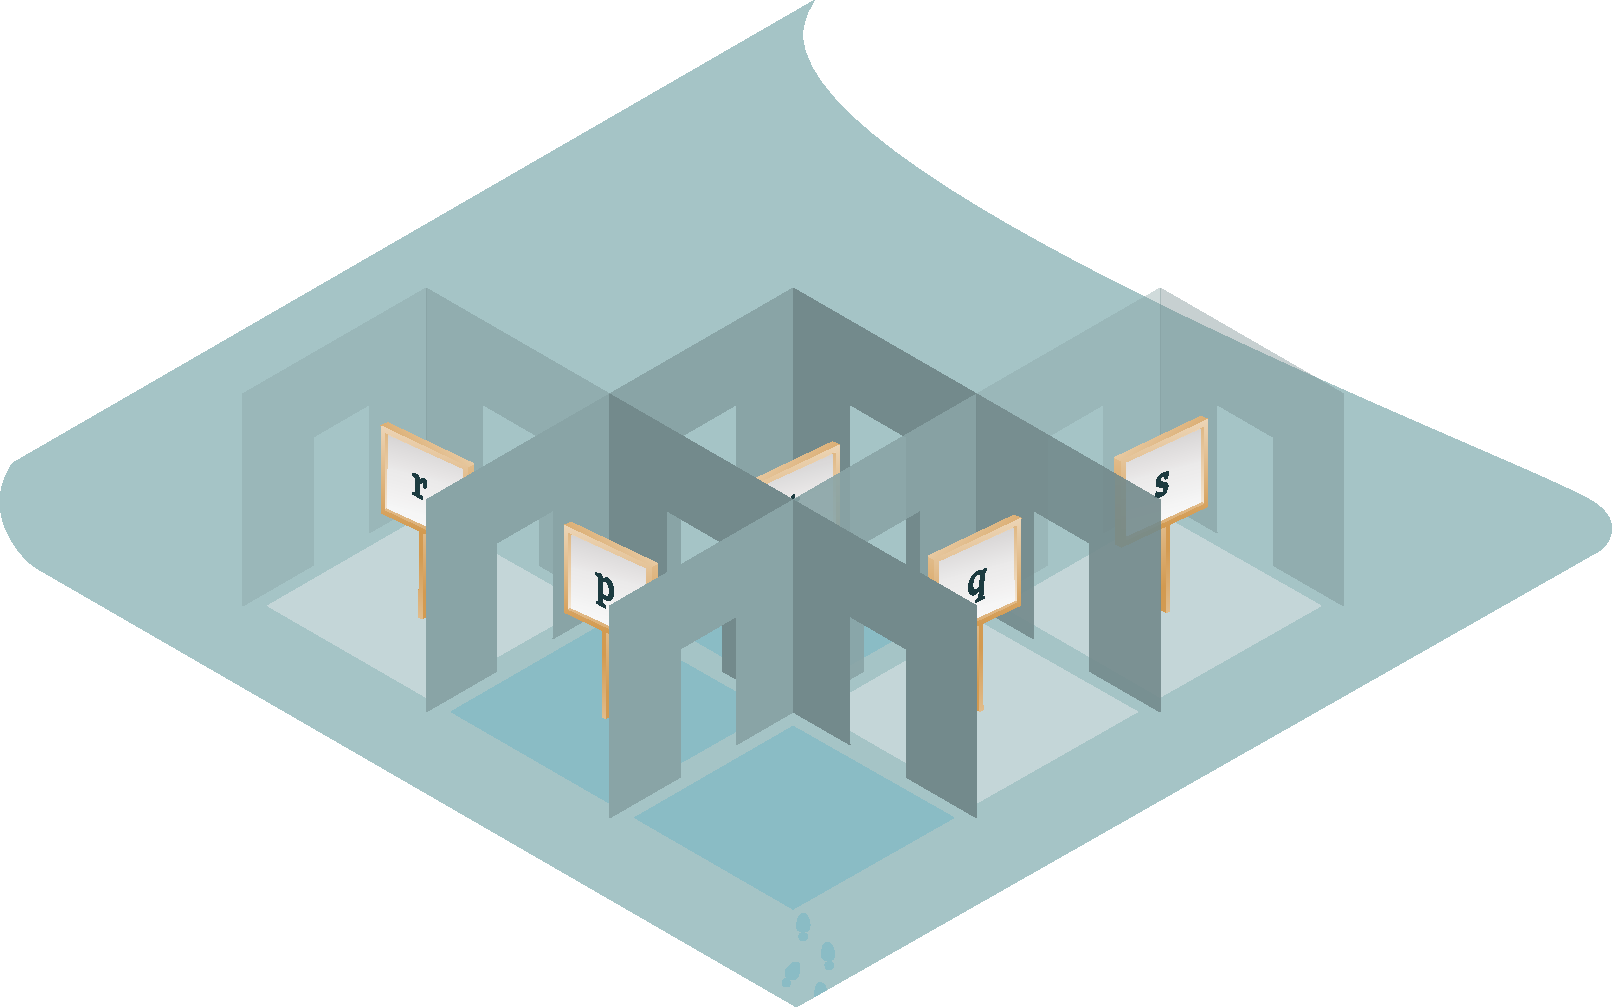
\includegraphics[keepaspectratio,alt={Passado, futuro, presente}]{img/pqr-cubicle-fs.pdf}}
\caption{Passado, futuro, presente}
\end{figure}

O utilitarismo fornece muitas ideias e conceitos interessantes. Por
exemplo, o princípio da ``utilidade marginal decrescente'' é útil para
diversos fins. Segundo esse princípio, a utilidade de um item diminui à
medida que a oferta de unidades aumenta (e vice-versa).

Por exemplo, quando você começa a se exercitar, no início o benefício é
grande e seus resultados melhoram dramaticamente. Mas quanto mais tempo
você continua treinando, menor o impacto de cada sessão individual. Se
você treina demais, a utilidade diminui e você começa a sofrer com os
sintomas de excesso de treino.

Outro exemplo: se você come uma bala, terá bastante prazer. Mas se comer
balas demais, pode ganhar peso e aumentar o risco de todo tipo de
doença. Esse paradoxo dos benefícios deve ser sempre lembrado quando
avaliamos as consequências das ações. O que é o bem comum agora pode não
ser o bem comum no futuro.

\begin{figure}
\centering
\pandocbounded{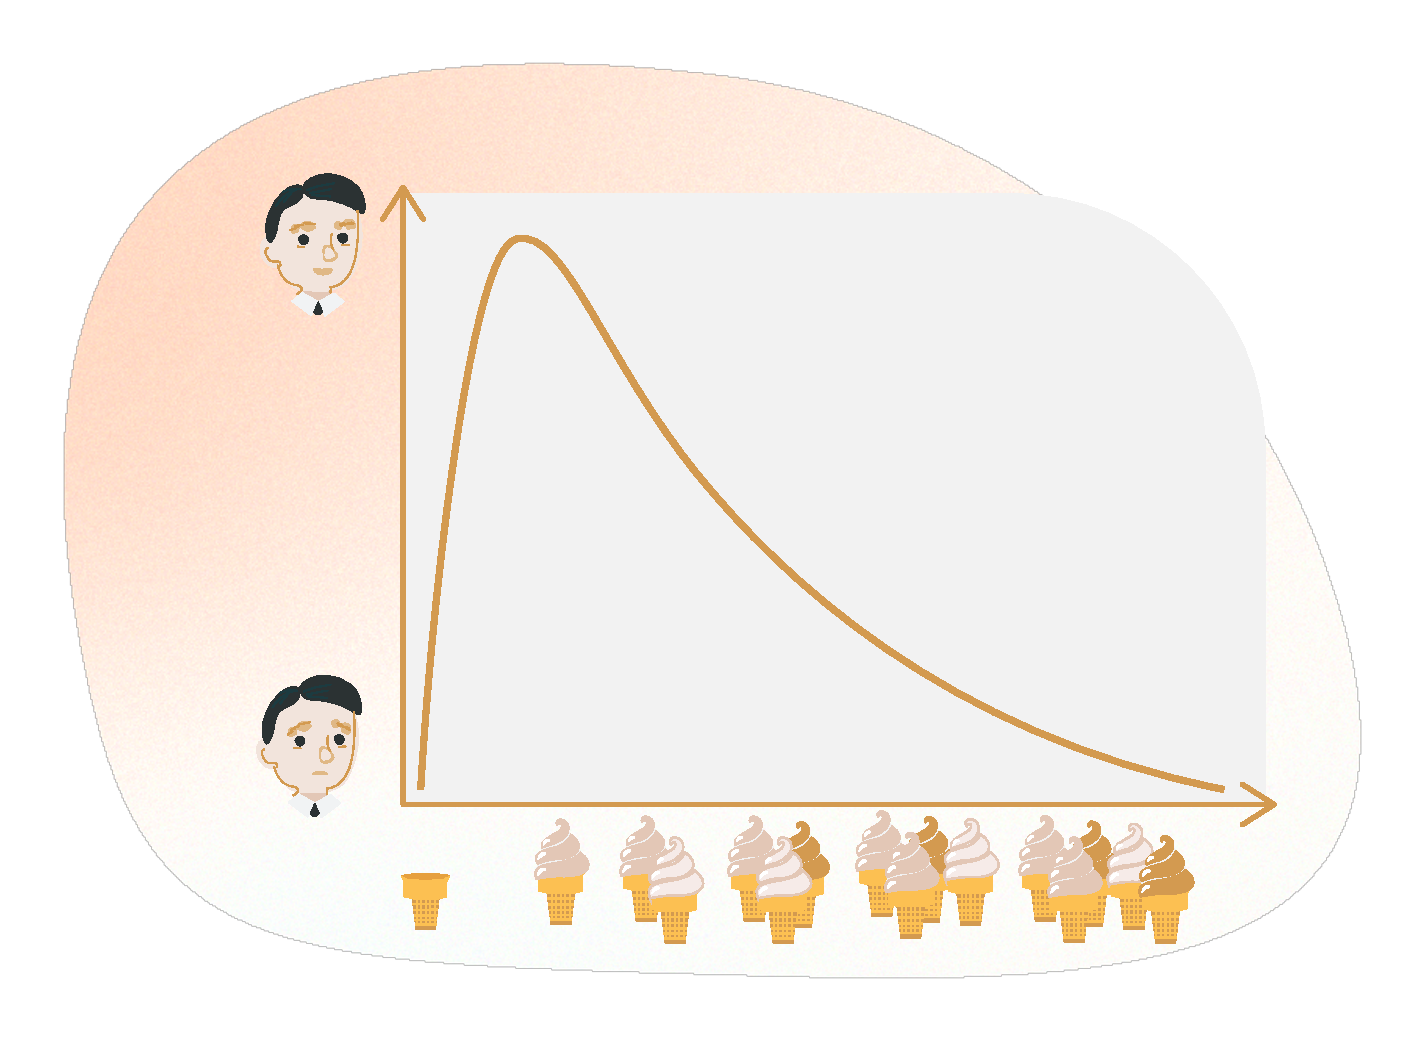
\includegraphics[keepaspectratio,alt={Utilidade marginal decrescente}]{img/dim-mu.pdf}}
\caption{Utilidade marginal decrescente}
\end{figure}

\subsection{III. Os problemas do
utilitarismo}\label{iii.-os-problemas-do-utilitarismo}

O utilitarismo não é uma explicação perfeita da tomada de decisão moral.
Ele foi criticado sob muitos aspectos. Por exemplo, o cálculo
utilitarista exige que atribuamos valores aos benefícios e danos
resultantes de nossas ações e os comparemos com as consequências que
poderiam resultar de outras ações. Mas frequentemente é difícil, senão
impossível, medir e comparar antecipadamente os valores de todos os
benefícios e custos relevantes.

``Risco'' é comumente usado para significar a probabilidade de um perigo
ou ameaça que surge de modo imprevisível ou, num sentido mais técnico, a
probabilidade de determinado grau de dano. Na ética da IA, entende-se
que danos e riscos surgem do projeto, da aplicação inadequada ou do uso
indevido intencional da tecnologia. Exemplos típicos são riscos como
discriminação, violação de privacidade, questões de segurança, guerra
cibernética ou invasão maliciosa. Na prática, é difícil comparar riscos
e benefícios pelas seguintes razões:

\textbf{Primeira:} riscos e benefícios são influenciados por
compromissos de valor, preferências subjetivas e diversas,
circunstâncias práticas e fatores pessoais e culturais.

\textbf{Segunda:} danos e benefícios não são estáticos. A utilidade
marginal de um item diminui de um modo que pode ser difícil de prever.
Além disso, um dano específico ou um benefício específico pode ter valor
de utilidade diferente em circunstâncias diferentes. Por exemplo, se um
carro mais rápido será ou não mais benéfico depende do uso pretendido
--- se a intenção é que seja um ônibus escolar, devemos priorizar a
segurança; se for usado como carro de corrida, a resposta pode ser
outra.

\textbf{Terceira:} as situações do mundo real costumam ser tão complexas
que é difícil prever ou comparar antecipadamente todos os riscos e
benefícios. Por exemplo, analisemos as possíveis consequências da
robótica militar. Embora os robôs militares contemporâneos sejam em
grande parte operados remotamente ou semiautônomos, com o tempo é
provável que se tornem totalmente autônomos. Segundo algumas
estimativas, os robôs reduzem as baixas civis e militares. Mas, segundo
outras, eles não reduzem o risco para os civis. Estatisticamente, nas
primeiras décadas de guerra do século XXI, armamentos robóticos
estiveram envolvidos em numerosas mortes tanto de soldados quanto de não
combatentes. A possibilidade de usar diversas técnicas --- como
\emph{adversarial patches} (adesivos adversariais, que interrompem a
capacidade de uma máquina de classificar imagens corretamente) --- para
enganar e manipular armas automatizadas complica a situação ao aumentar
o risco específico de causar dano a civis. O nível geral de risco também
depende da facilidade com que guerras poderiam ser declaradas caso os
robôs assumam a maior parte do risco físico.

\textbf{Quarta:} o utilitarismo não leva em conta outros aspectos
morais. É fácil imaginar situações em que uma tecnologia desenvolvida
produziria grandes benefícios para as sociedades, mas cujo uso ainda
assim levantaria questões éticas importantes. Por exemplo, pensemos no
caso de um sistema de saúde preventiva. O sistema pode de fato ser
benéfico para muitos, mas ainda nos obriga a perguntar se direitos
humanos fundamentais, como a privacidade, importam. Ou o que acontece
com o direito do cidadão de \emph{não} saber sobre possíveis problemas
de saúde? (Muitos de nós gostaríamos de saber se estamos num grupo de
alto risco, mas e se alguém não quiser saber? Pode uma cidade impor esse
conhecimento a essa pessoa?) Ou ainda: como garantir que todos tenham
acesso igual aos possíveis benefícios de um sistema preventivo?

\begin{filosofia}[O monstro de utilidade de Nozick]

Uma das maiores dificuldades do utilitarismo é a questão da utilidade: o
que ela é, afinal? Tecnicamente, utilidade é apenas uma medida (uma
quantidade numérica) que descreve algum tipo de ``bem'' subjacente que
queremos maximizar. Digamos, prazer ou bem-estar (que filósofos
hedonistas afirmariam ser a mesma coisa). O prazer é, ao menos em certa
medida, uma experiência subjetiva, e a utilidade, como medida, deveria
transformá-lo num número comparável entre sujeitos. Essa é uma exigência
elevada.

Supondo que tal medida de utilidade de fato exista, o filósofo Robert
Nozick apresenta o seguinte enigma. Existe uma criatura chamada Monstro
de Utilidade. Sua mente hedonista é constituída de tal forma que, dado
qualquer recurso, ela obtém dele mais prazer do que qualquer outro
indivíduo obteria. Ela simplesmente aprecia maçãs, carros, café,
liberdade etc. mais do que qualquer outra pessoa. Isso significa que ela
extrai mais utilidade dessas coisas, e se somos moralmente obrigados a
maximizar a utilidade produzida pelos recursos que temos, a conclusão é
clara: tudo o que temos vai para o Monstro de Utilidade. Nada para mais
ninguém.

Isso torna o utilitarismo indefensável? Existe algum modo de o
utilitarista argumentar que o enigma proposto por Nozick não é realmente
um problema?

\end{filosofia}

\begin{reflexao}[Exercícios desta seção]

O material original traz aqui um questionário interativo. As perguntas
não constam do repositório de origem --- ficam no banco de dados da
plataforma. O exercício correspondente deve ser redigido em
\texttt{exercicios/capitulo02-exercicios.md}.

\end{reflexao}

\subsection{IV. Bem comum e bem-estar}\label{iv.-bem-comum-e-bem-estar}

Apesar dos problemas descritos na seção anterior, os princípios do
utilitarismo podem nos ajudar a considerar as consequências imediatas e
as menos imediatas de nossas ações. Convém lembrar que, na vida real,
definir o ``bem comum'' exige uma diversidade de pontos de vista.

\begin{filosofia}[O que é bem-estar?]

Com frequência, o termo ``bem comum'' é tomado como sinônimo de
``bem-estar''. Mas o que é bem-estar? As raízes da pesquisa sobre
bem-estar estão na Grécia antiga, onde filósofos como Aristóteles se
concentravam em como alcançar ``a boa vida''. Desde então, a busca pela
boa vida tem sido tema constante em diferentes disciplinas. Hoje, a
pesquisa em campos como psicologia, economia e ciências sociais aborda o
bem-estar em termos ``das dimensões biológica, pessoal, relacional,
institucional, cultural e global da vida''. Essas dimensões abrangem
fatores como vitalidade física e mental, satisfação social e senso de
realização e plenitude pessoal.

Os estudos sobre bem-estar podem ser divididos em três subtipos
principais:

\textbf{1) As teorias subjetivas.} Concentram-se em questões como o modo
que as pessoas se sentem ao longo da vida cotidiana, ou como uma pessoa
avalia a própria vida. Esse tipo de bem-estar psicológico é
frequentemente descrito como a experiência de alta satisfação com a
vida, altos níveis de emoções e humores agradáveis e baixos níveis de
emoções e humores negativos.

\textbf{2) As teorias eudaimônicas.} Consideram o bem-estar
principalmente como resultado da busca de objetivos positivos. A
perspectiva eudaimônica diferencia o bem-estar da satisfação do desejo.
Segundo essas teorias, bem-estar e felicidade subjetiva não devem ser
equiparados, porque os resultados produtores de prazer que fundamentam a
felicidade subjetiva não necessariamente promovem saúde e bem-estar. Em
vez disso, entende-se que o bem-estar requer componentes como autonomia,
domínio do ambiente, crescimento pessoal, relações positivas com os
outros, senso de propósito na vida e autoaceitação. Essas dimensões
descrevem o bem-estar como uma avaliação globalmente positiva de si
mesmo, a aceitação da própria história de vida e dos talentos
individuais como membro de uma comunidade, a crença de que a própria
vida é significativa e um senso de autodeterminação.

\textbf{3) As teorias sociais.} Nelas, o bem-estar é abordado em termos
de fatores sociais, como integração, contribuições à vida social,
coerência social e aceitação social. O bem-estar depende do grau em que
um indivíduo funciona bem em seus ambientes sociais.

Hoje, muitas das abordagens do bem-estar combinam elementos de todas
essas teorias. O bem-estar é visto como uma combinação complexa de
aspectos psicológicos, sociais e físicos, e adota uma perspectiva de
qualidade de vida como um todo.

Pesquisas como o \emph{World Happiness Report} são exemplos dessa
abordagem holística. O relatório é uma publicação anual da Rede de
Soluções para o Desenvolvimento Sustentável das Nações Unidas. Contém
artigos e classificações de felicidade nacional baseadas na avaliação
que os respondentes fazem da própria vida, que o relatório também
correlaciona com diversos fatores de vida. (Até março de 2020, a
Finlândia foi classificada como o país mais feliz do mundo três vezes
seguidas.)

Além disso, pesquisadores desenvolvem constantemente novas maneiras de
abordar o bem-estar. Por exemplo, os grandes volumes de dados (\emph{big
data}) são hoje utilizados de muitas formas na pesquisa sobre bem-estar.
Os métodos contemporâneos incluem a análise mais avançada de dados
demográficos e socioeconômicos, mas também, por exemplo, o uso de
ferramentas de mineração de texto em documentos escritos --- como
publicações no Twitter, no Facebook ou outros dados de redes sociais
---, além da análise de pegadas digitais e até de traços faciais.

\end{filosofia}

A abordagem do bem comum exige que todos tenham acesso aos benefícios da
IA. Isso destaca a importância de assegurar que os benefícios potenciais
da IA não se acumulem de forma desigual e sejam tornados acessíveis ao
maior número possível de pessoas. Além disso, a IA deve estar alinhada a
valores, objetivos e normas, respeitando em grau suficiente a
diversidade cultural e individual.

O bem comum não é um singular, mas um plural. Identificar as normas
sociais e morais da comunidade específica em que uma IA será implantada
é, portanto, obrigatório. É o único caminho para levar à sociedade os
benefícios potencialmente significativos e diversos da IA e para
promover, entre outras coisas, maior bem-estar e assistência social para
todos.

\begin{reflexao}[Exercícios desta seção]

O material original traz aqui dois questionários interativos. As
perguntas não constam do repositório de origem. Os exercícios
correspondentes devem ser redigidos em
\texttt{exercicios/capitulo02-exercicios.md}.

\end{reflexao}

\subsection{Referências}\label{referuxeancias}

Bentham, J. (1789). \emph{An Introduction to the Principles of Morals
and Legislation}.

Mittelstadt, B. (2019). Principles alone cannot guarantee ethical AI.
\emph{Nature Machine Intelligence}, 1, 501--507.

Morozov, E. (2013). \emph{To Save Everything, Click Here: The Folly of
Technological Solutionism}. PublicAffairs.

Nozick, R. (1974). \emph{Anarchy, State, and Utopia}. Basic Books.

\emph{World Happiness Report}. UN Sustainable Development Solutions
Network. \url{https://worldhappiness.report/}

\begin{center}\rule{0.5\linewidth}{0.5pt}\end{center}

\begin{licenca}

\textbf{Material original:} \emph{Ethics of AI}, um curso online
gratuito da Universidade de Helsinque. Professores responsáveis:
Anna-Mari Rusanen e Jukka K. Nurminen. Demais contribuintes principais:
Santeri Räisänen, Sasu Tarkoma e Saara Halmetoja. Disponível em
\url{https://ethics-of-ai.mooc.fi/}.

\textbf{Esta versão:} tradução e adaptação para o português brasileiro
realizada por José Lucas Lira Bizil, Fernando Mazzeto Lisboa Lima e
Matheus da Silva Fernandes, no âmbito do Programa CiberExt 26-29
(FEELT38103), Universidade Federal de Uberlândia, 2026. Esta é uma obra
derivada; os autores originais não a revisaram nem a endossam.

\textbf{Licença:} Creative Commons
Atribuição-NãoComercial-CompartilhaIgual 4.0 Internacional (CC BY-NC-SA
4.0) ---
\url{https://creativecommons.org/licenses/by-nc-sa/4.0/deed.pt-br}.

\end{licenca}

\end{document}
